\subsection{Credit Derivatives}

\begin{definition} \hlt{Credit Derivatives}\\
Derivative instrument where the underlying is a measure of borrower's credit quality.\\
Includes total return swaps, credit spread options, credit-linked notes, credit default swaps (CDS).
\end{definition}

\subsubsection{Credit Default Swaps}

\begin{definition} \hlt{Credit Default Swap (CDS)}\\
Underlying is the credit quality of a borrower. Credit protection buyer (short credit risk and CDS) gets compensated by credit protection seller (long credit risk and CDS) through paying CDS spread to seller.
\end{definition}

\begin{figure}[H]
\centering
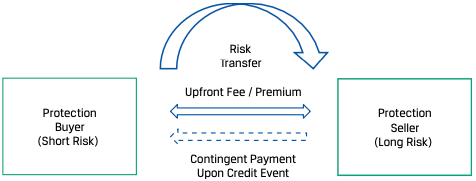
\includegraphics[scale=0.45]{/fi/cdspayment}
\caption{Payment structure of CDS}
\end{figure}

\begin{remark} \hlt{Credit Events}\\
Credit events covered may include bankruptcy, failure to pay, restructuring.\\
Sovereign and municipal bond may have moratorium, or repudiation of debt where the government authority declares a moratorium on payments due under the terms of obligation, or challenges the validity of the entire debt obligation. Succession event occurs when there is a change in corporate structure of reference entity.\\
A $15$-member group of ISDA called the Determinations Committee (DC) is required to have supermajority vote ($>12$ members) for a credit event to be declared.
\end{remark}

\begin{definition} \hlt{Single-Name CDS}\\
CDS on one specific entity. Borrower is the reference entity, fixed-income security 	on which the swap is written is the reference obligation, and the contract specifies a reference obligation.\\
The designated instrument is usually a senior unsecured obligation.\\
CDS pay offs only when reference entity defaults on any other issue that is ranked pari passu or higher.\\
CDS payoff is based on market value of cheapest-to-deliver (CTD) bond (debt instrument with same seniority as reference obligation but can be purchased and delivered at lowest code).
\end{definition}

\begin{definition} \hlt{Index CDS}\\
Covers multiple issuers, allow market participants to take exposure on credit risk of several companies simultaneously. Protection for each issuer is equally weighted, total notional capital is sum of protection on all issuers. Pricing is dependent on credit correlation; the more correlated the defaults, the more costly the index CDS.\\
When entity in index defaults, it is removed from index and settled as a single-name CDS based on its relative proportion in the index. The index moves forward with smaller notional.\\
Index CDS are used to take positions on credit risk of sectors covered, and protect bond portfolio which consists of or are similar to components of the indexes.
\end{definition}

\begin{definition} \hlt{Tranche CDS}\\
Covers a combination of borrowers but only up to pre-specified level of losses.
\end{definition}

\begin{remark} \hlt{International Swaps and Derivatives Association (ISDA) Master Agreement}\\
Specifications which parties to CDS contracts conform to.
\end{remark}

\begin{remark} \hlt{Features of CDS Contract}\\
Each CDS contract specifies a notional amount (amount of protection being purchased), which can be thought of as size of contract. Total notional amount can exceed debt outstanding of reference entity.\\
Typical maturity range is 1 to 10 years, but two parties can negotiate any maturity.\\
Standard annual coupon rates are $1\%$ and $5\%$, where buyer makes quarterly payments. Difference between credit spread and standard rate is converted to present value basis, and buyer/seller makes upfront premium.
\end{remark}

\begin{remark} \hlt{Settlement Protocol}\\
Settlement typical occurs 30 days after declaration of credit event, by physical or cash settlement.\\
In physical settlement, seller receives the reference obligation (bond or loan) and pays buyer the notional.\\
In cash settlement, seller pays buyer according to recovery rate.
\begin{align}
\text{Payout Amount} &= \text{LGD} \times \text{Notional} \nonumber \\
\text{LGD} &= 1 - \text{Recovery Rate} \nonumber
\end{align}
\end{remark}

\begin{remark} \hlt{Valuation of CDS}\\
CVA is a reasonable approximation for a CDS hedge position that would give investor a risk-free rate of return.\\
Method of computing CDS Spread is largely similar to CVA in Method \ref{method:computingcva}, to compute RR and POD.
\begin{equation}
\text{CDS Spread} \approx (1-\text{RR}) \times \text{POD} \nonumber
\end{equation}
Cash payments made by buyer on CDS cease when there is a default. Hence expected value of coupon payments also depends on hazard rate.\\
Payments from buyer to seller are the premium leg. In case of default, seller makes payment to buyer with contingent payments, which make up the protection leg.
\begin{equation}
\text{Buyer Upfront Payment} = PV(\text{Protection Leg}) - PV(\text{Premium Leg}) \nonumber
\end{equation}
Upfront premium may be approximated as difference between CDS spread and CDS coupon rate, multiplied by duration of CDS. The CDS spread is compensation for bearing credit risk of reference obligation.
\begin{align}
\text{Upfront Premium}\% \approx (\text{CDS Spread} - \text{CDS Coupon}) \times \text{Duration} \nonumber
\end{align}
\end{remark}

\begin{figure}[H]
\centering
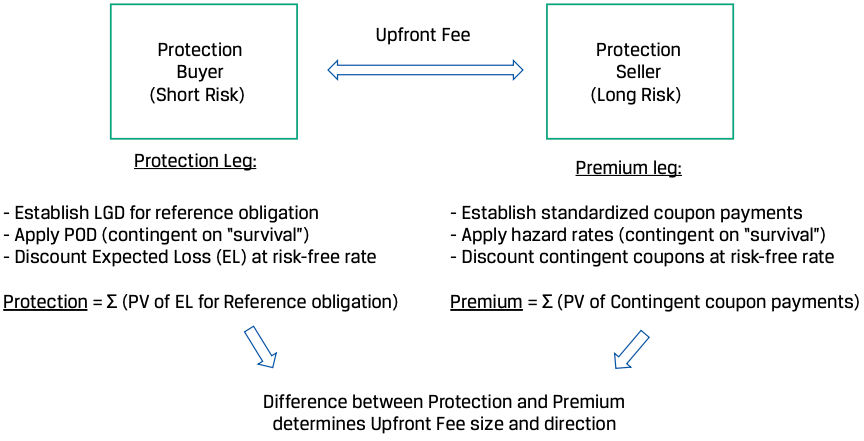
\includegraphics[scale=0.45]{/fi/cdspropreleg}
\caption{Determination of CDS protection and premium legs}
\end{figure}

\begin{definition} \hlt{Credit Curve}\\
Credit spreads for range of maturity of company's debt, as determined by CDS rates.\\
Constant hazard rate will flatten the curve, but curve will not be completely flat due to discounting.\\
Upward-sloping credit curves imply greater probability of default in later years, downward-sloping are a result of severe near-term stress in financial markets
\end{definition}

\begin{remark} \hlt{Valuation Changes in CDS Over Bond Life}\\
At inception, the CDS spread and upfront premium is computed based on credit quality of reference entity.\\
After inception, credit quality of reference entity and credit risk premium in overall market may change, leading to underlying CDS having non-zero value. If credit spread declines, seller (locked in higher credit spread at initiation) would gain.\\
Change in value of CDS after inception approximated by change in spread multiplied by duration of CDS.
\begin{align}
\text{P\&L for Protection Buyer} &\approx \Delta\text{Spread} \times \text{Duration} \times \text{Notional} \nonumber \\
\text{\% Change in CDS Price} &\approx \Delta\text{Spread in bps} \times \text{Duration} \nonumber
\end{align}
Note protection buyer is short credit risk, hence benefits when credit spreads widen.
\end{remark}

\begin{remark} \hlt{Monetising Gains and Losses of CDS}\\
Protection buyer or seller may unwind an existing CDS exposure prior to expiration or default by entering into an offsetting transaction with same terms as original CDS and maturity equal to remaining maturity on existing CDS. Difference between upfront premium paid and received is approximately equal to profit for protection buyer. This process of capturing value from in-the-money CDS exposure is monetising the gain.
\end{remark}

\begin{remark} \hlt{CDS for Managing Portfolio Credit Exposure}\\
Lender buy protection to reduce its credit exposure to a borrower, as lender may have assumed too much credit risk but does not want to sell the bond or loan due to significant transaction costs, or the bond is illiquid. If risk is temporary, it is easier to temporary reduce risk by using CDS.\\
Seller objective is to profit from market making in CDS. Exposure may be managed by diversifying credit risks or hedging the risk by entering the transaction into another party (i..e, shorting the debt or equity of reference entity), with investment of the funds in a repurchase agreement.\\
Alternatively, a bondholder is a buyer of credit and interest rate risk. If only credit risk is wanted, then protection is sold, which would require less capital and transaction cost than buying the bond. CDS may be more liquid than the bond, hence position can be unwounded more easily. 
\end{remark}

\begin{remark} \hlt{Naked CDS}\\
Investor with no underlying exposure buys or sells protection.\\
Investor is taking position that entity's credit quality will improve.
\end{remark}

\begin{remark} \hlt{Long/Short Credit Trade}\\
Investor buys protection on one reference entity while selling protection on another (related) reference entity.\\
Investor is betting that the difference in credit spreads between two reference entities will change advantageously.\\
Investor may also long/short CDS indexes. In recession, buy protection with high-yield CDS index and sell protection on investment-grade CDS index. As high-yield spreads widen relative to investment-grade spreads, the trade would realise a profit.
\end{remark}

\begin{remark} \hlt{Curve Trade}\\
Investor buys protection at one maturity and sell protection on same reference entity at difference maturity.\\
If upward-sloping yield curve becomes steeper, long-term credit risk increases relative to short-term credit risk; investor buy long-term duration and sell short-term duration. In the short-run, curve-steeping trade is bullish, as short-term outlook for reference entity is better than long-term outlook. Vice versa for curve-flattening case.
\end{remark}

\begin{remark} \hlt{Strategy for Shift in Level of Curve}\\
If all spreads is expected to go up, investor to buy protection at the long-term, and sell protection at the short-term, as longer-term CDS will move more than short-term CDS.
\end{remark}

\begin{remark} \hlt{Basis Trade}\\
Attempt to exploit difference in credit spreads between bond markets and CDS market.\\
Mis-pricing will be temporary and the disparity should eventually disappear.\\
If credit spread in bond market is higher than CDS spread on same bond, buy the bond and take buyer protection position in CDS market. If convergence occurs, investor makes profit.
\end{remark}

\begin{remark} \hlt{Arbitrage on Same Name Entity Instruments}\\
Investor to use CDS market to first determine if any of the instruments of the single reference entity is priced incorrectly relative to the CDS, then buy the cheaper instrument and sell the more expensive instrument.\\
Assumes the market will adjust. More complex to execute, as priority of claims mean not all instruments pay off equally if default occurs.
\end{remark}

\begin{remark} \hlt{Arbitrage on CDS Indexes}\\
If cost of index is not equivalent to aggregate cost of index components, investor to long cheaper instrument and short more expensive instrument.\\
Assumes convergence will occur. Investor gains profit while neutralising the risk.\\
Transaction costs may be significant and hence nullify the profit potential.
\end{remark}

\begin{remark} \hlt{LBO-Event Investment}\\
In LBO, firm issues great amount of debt to repurchase all of target's public equity, which increases CDS spread as default is more likely. Investor who anticipates an LBO to purchase both stock and CDS protection, both of which will increase in value when LBO occurs.
\end{remark}

\begin{remark} \hlt{Synthetic CDO Arbitrage}\\
CDSs are claims against portfolio of debt securities. Synthetic CDO has similar credit risk exposure to cash CDO, but assembled with CDS. If Synthetic CDO can be created at lower cost than cash CDO, investor to buy synthetic CDO and sell the cash CDO, hence profiting from the arbitrage.
\end{remark}
